% ============================================================
% GP-109 Research Paper — LaTeX Source
% Title: Can an AI Explanation Be Misused?
%        Testing Whether SHAP and LIME Help Patients Game
%        a Clinical Diabetes Risk Model
%
% Target venue: FAccT 2028 / AIES 2028
% Template: ACM Conference Proceedings
% ============================================================

\documentclass[sigconf,nonacm]{acmart}

% ---- Packages ------------------------------------------------
\usepackage{booktabs}       % professional tables
\usepackage{microtype}      % better typography
\usepackage{graphicx}       % figures
\usepackage{subcaption}     % subfigures
\usepackage{amsmath}        % math
\usepackage{amssymb}
\usepackage{hyperref}       % clickable refs (disable for camera-ready)
\usepackage{cleveref}       % \cref
\usepackage{xcolor}
\usepackage{multirow}
\usepackage{array}

% ---- Metadata ------------------------------------------------
\title{Can an AI Explanation Be Misused? Testing Whether SHAP and LIME
       Help Patients Game a Clinical Diabetes Risk Model}

\author{Akash Singh}
\affiliation{%
  \institution{Delhi Technological University}
  \city{Delhi}
  \country{India}
}
\email{akash@dtu.ac.in}

\author{Aditya Jha}
\affiliation{%
  \institution{Delhi Technological University}
  \city{Delhi}
  \country{India}
}
\email{aditya@dtu.ac.in}

\author{Akshat Kumar}
\affiliation{%
  \institution{Delhi Technological University}
  \city{Delhi}
  \country{India}
}
\email{akshat@dtu.ac.in}

% ---- Abstract -----------------------------------------------
\begin{abstract}
Explainable AI (XAI) methods such as SHAP and LIME are increasingly
required by regulation to accompany machine learning predictions in
healthcare. A concern is that feature attributions may also serve as
instructions for gaming the model---telling a patient exactly which
self-reported inputs to adjust for a better risk score. However, a
determined adversary can also simply query the model repeatedly with
different inputs and observe the score change. We compare these two
adversarial strategies on a diabetes risk model trained on NHANES
public health survey data, constraining the adversary's permissible
lies to magnitudes observed in real self-reporting behaviour. We train
four models---two algorithms (Random Forest, Logistic Regression)
$\times$ two input variants (nurse-measured vs.\ self-reported
height/weight)---and measure how many blind trial-and-error attempts
equal one explanation in terms of achieved score reduction: the
\emph{explanation equivalence} $N^*$. Our pre-registered experiment on
the held-out 2017--2018 NHANES cycle finds that one SHAP explanation is
equivalent to approximately $N^*$ blind attempts [95\% CI: $L$--$H$],
suggesting that explanations provide only a \textbf{[small/moderate]}
additional advantage over informed trial-and-error. Crucially, for the
majority of patients the explanation provides zero benefit over a single
random query, implying that withholding XAI explanations is not an
effective safeguard---verifying patient-reported inputs is more
impactful. We release our code and pre-registered analysis plan.

\textbf{Note:} Values in brackets [$N^*$, $L$, $H$] will be filled
with final experiment results from Stage 7.
\end{abstract}

% ---- CCS Concepts / Keywords --------------------------------
\begin{CCSXML}
<ccs2012>
  <concept>
    <concept_id>10010147.10010257.10010293</concept_id>
    <concept_desc>Computing methodologies~Machine learning</concept_desc>
    <concept_significance>500</concept_significance>
  </concept>
  <concept>
    <concept_id>10003456.10003462</concept_id>
    <concept_desc>Social and professional topics~Medical records</concept_desc>
    <concept_significance>300</concept_significance>
  </concept>
</ccs2012>
\end{CCSXML}

\ccsdesc[500]{Computing methodologies~Machine learning}
\ccsdesc[300]{Social and professional topics~Medical records}

\keywords{explainability, SHAP, LIME, adversarial, gaming, diabetes,
          NHANES, clinical AI, transparency, fairness}

\maketitle

% ============================================================
\section{Introduction}
% ============================================================

The deployment of machine learning models in high-stakes clinical
settings has prompted widespread calls for transparency.  Regulations
such as the EU AI Act and GDPR's ``right to explanation'' push
developers to provide explanations alongside predictions
\cite{goodman2017european}.  In diabetes risk prediction, a model
might inform a patient: ``Your risk score is 0.72. Your weight is the
most important contributing factor.''

% --- TODO (Akash Singh, Week 2) ----------------------------
% 1.5 pages. Cover:
%   - The dual-use tension: transparency ↔ gaming
%   - Concrete example: patient adjusts self-report after seeing explanation
%   - Prior work gap: gaming studied for images/text, not for clinical
%     self-report bias models
%   - Our contribution (4 bullets)
%   - Paper roadmap (1 paragraph)

This transparency creates a potential dual-use risk: the same
explanation that helps a clinician understand the model may help a
patient \emph{game} it by adjusting what they self-report.  A patient
told that weight is the top risk factor might under-report their weight
at the next visit.

\paragraph{Our Question.}
Does a SHAP or LIME explanation give a patient a meaningful advantage
over simply trying different inputs until the score improves---i.e.,
blind trial-and-error?  If explanations provide only a small advantage,
restricting them is not an effective safeguard.  If they provide a
large advantage, the benefit of transparency must be weighed against
the gaming risk.

\paragraph{Contributions.}
\begin{enumerate}
  \item We introduce \emph{explanation equivalence} ($N^*$): the
        number of blind attempts required to achieve the same score
        reduction as one explanation.
  \item We operationalise a realistic \emph{lie budget} from real
        NHANES self-reporting data, bounding the adversary's
        permissible misreporting magnitudes.
  \item We conduct the first \emph{pre-registered} adversarial
        evaluation of SHAP and LIME on a real clinical dataset,
        preventing p-hacking and HARKing.
  \item We provide actionable policy conclusions: whether restricting
        explanations is an effective safeguard.
\end{enumerate}

% ============================================================
\section{Related Work}
% ============================================================

% --- TODO (Akash Singh, Week 2) ----------------------------
% 1.5 pages. Cite and position:
%   [1] Ribeiro et al. LIME (2016)
%   [2] Lundberg & Lee SHAP (2017)
%   [3] Adadi & Berrada XAI survey (2018)
%   [4] Shokri et al. privacy in XAI (AIES 2021)
%   [5] Ghalme et al. strategic classification (ICML 2021)
%   [6] Slack et al. fooling LIME/SHAP (AAIS 2020)
%   [7] Goodman & Flaxman GDPR (2017)
%   [8] Wachter et al. counterfactual explanations (2017)
%   [9] Johnson et al. NHANES data (2014)
% Distinguish: our work tests gaming, not model-level attacks.
% Distinguish: our lie budget comes from real human misreport data.

\paragraph{Explainability Methods.}
Local explanation methods such as LIME~\cite{ribeiro2016lime} and
SHAP~\cite{lundberg2017shap} produce feature attributions that
identify the most important inputs for a given prediction.  These
methods are increasingly embedded in clinical decision support
systems~\cite{adadi2018peeking}.

\paragraph{Adversarial XAI.}
Slack et al.~\cite{slack2020fooling} demonstrated that SHAP and LIME
can be manipulated at the \emph{model} level to produce misleading
explanations.  Our work is complementary: we study gaming at the
\emph{user} level, asking whether an honest model's explanations help
a user game their score.

Shokri et al.~\cite{shokri2021privacy} showed that explanations can
leak private training data.  Ghalme et al.~\cite{ghalme2021strategic}
studied strategic classification where agents best-respond to a known
model; we study the more realistic setting where the model is a black
box and the lie budget is bounded by real human behaviour.

\paragraph{Self-Reporting Bias.}
NHANES~\cite{johnson2014national} systematically collects both
self-reported and nurse-measured anthropometrics, enabling a direct
empirical measurement of the lie budget.

% ============================================================
\section{Problem Setup}
% ============================================================

% --- TODO (Aditya Jha, Week 2) ----------------------------
% 1 page. Formal definitions:
%   - Model f: X → [0,1], diabetes risk score
%   - Gameable features G ⊂ X (self_height_cm, self_weight_kg)
%   - Lie budget B(g) = max permissible |x_g' - x_g|
%   - Strategy 1: explanation-guided attack
%   - Strategy 2: blind trial-and-error
%   - Equivalence metric N*
%   - Threat model

\subsection{Threat Model}

We model an adversary who:
\begin{itemize}
  \item Receives a diabetes risk score $f(\mathbf{x}) \in [0,1]$ from
        a clinical AI system.
  \item Can modify self-reported features $G = \{\text{height},
        \text{weight}\}$ by at most $B(g)$ (the \emph{lie budget}).
  \item Wishes to minimise their score while staying within the lie
        budget (i.e., the misreport is plausible).
  \item May or may not receive a SHAP/LIME explanation.
\end{itemize}

\subsection{Lie Budget}

The lie budget is derived empirically from NHANES: for each gameable
feature $g$, we compute $B(g) = \text{Percentile}_{95}(|x_g^{\text{self}}
- x_g^{\text{measured}}|)$ using the 2015--2016 development cycle.
This gives $B(\text{height}) = 7.29\,\text{cm}$ and
$B(\text{weight}) = 8.96\,\text{kg}$.

\subsection{Explanation Equivalence}

\begin{definition}[Explanation Equivalence $N^*$]
Let $R_{\text{exp}}$ be the mean score reduction achieved by the
explanation-guided strategy.  Let $R_{\text{blind}}(N)$ be the mean
score reduction achieved by the blind strategy with $N$ attempts.
The \emph{explanation equivalence} is:
\[
  N^* = \inf \{ N \geq 0 : R_{\text{blind}}(N) \geq R_{\text{exp}} \}
\]
estimated by linear interpolation on the curve
$N \mapsto R_{\text{blind}}(N)$.
\end{definition}

% ============================================================
\section{Methodology}
% ============================================================

% --- TODO (Aditya Jha, Week 3) ----------------------------
% 2 pages. Sub-sections:
%   4.1 Dataset & preprocessing (NHANES, N=X patients, 12.4% diabetes)
%   4.2 Models (RF, LR — hyperparameters from Table 2)
%   4.3 Explanation methods (TreeSHAP, LIME config)
%   4.4 Adversarial strategies (Algorithm 1 pseudocode)
%   4.5 Statistical analysis (Wilcoxon, bootstrap CI)
%   4.6 Pre-registration

\subsection{Dataset}

We use the NHANES public health survey~\cite{johnson2014national},
which collects both nurse-measured and self-reported anthropometrics.
We merge the demographic, examination, and laboratory components for
the 2015--2016 (development) and 2017--2018 (held-out test) cycles.
After retaining adults ($\geq$18 years) with complete records across
all features, we obtain $N_{\text{dev}} = $ [FILL] patients
(2015--2016) and $N_{\text{test}} = 884$ patients (2017--2018),
with diabetes prevalence (HbA1c $\geq 6.5\%$) of [FILL]\% and
[FILL]\%, respectively.

\subsection{Models}

We train two model types---Random Forest (RF, $n=100$ trees,
$\text{max\_depth}=10$) and Logistic Regression (LR)---each in two
variants: \emph{Model A} uses nurse-measured height/weight;
\emph{Model B} uses self-reported values (see Table~\ref{tab:model_perf}).
All hyperparameters were fixed before examining the held-out data
(see Section~\ref{sec:preregistration}).

\subsection{Adversarial Strategies}

\paragraph{Strategy 1 (Explanation-Guided).}
The adversary requests one SHAP or LIME explanation, identifies the
most influential gameable feature, and adjusts it by $B(g)$ in the
risk-reducing direction (Algorithm~1 in Supplementary).

\paragraph{Strategy 2 (Blind Trial-and-Error).}
The adversary makes $N$ sequential model queries, each with a
uniformly random perturbation of a gameable feature within $B(g)$,
keeping the best score found.  We evaluate $N \in \{1, 2, 3, 5, 10,
15, 20, 30, 50, 100\}$.

\paragraph{Key Design Choice.}
The blind simulation is run \emph{once} up to $N_{\max}=100$,
recording the running best at each milestone.  Running independent
simulations per $N$ would over-estimate blind performance at large $N$
and bias $N^*$ upward.

\subsection{Statistical Analysis}

For each configuration we compute: (i) mean $N^*$ with 1000-iteration
bootstrap 95\% CI; (ii) a paired Wilcoxon signed-rank test comparing
per-patient explanation vs.\ blind reductions at $N=10$;
(iii) Cohen's $d$ effect size.

\subsection{Pre-Registration}
\label{sec:preregistration}

The complete analysis plan---including all hypotheses, metric
definitions, and expected results---was published at
\url{https://github.com/GP109-DTU/btp} (git tag:
\texttt{v0.1-preregistration}) before the held-out 2017--2018 data
was processed.  All deviations from the plan are documented in a
changelog.

% ============================================================
\section{Experiments and Results}
% ============================================================

% --- TODO (Akshat Kumar, Week 3) ---------------------------
% 2 pages. Sub-sections:
%   5.1 Reporting gap (Table 3 + Fig 1)
%   5.2 Model performance (Table 2)
%   5.3 Main result: equivalence N* (Table 4 + Fig 2)
%   5.4 Per-patient distribution (Fig 7)
%   5.5 Model A vs Model B (Table 6 + Fig 4)
%   5.6 SHAP vs LIME agreement (Fig 5)
%   5.7 Statistical tests (Table 5)

\subsection{Reporting Gap}

Figure~\ref{fig:gaps} shows the distribution of self-reported minus
nurse-measured values in the 2017--2018 holdout data.  On average,
participants overestimate their height by $[X]$\,cm (SD $[Y]$) and
underestimate their weight by $[X]$\,kg (SD $[Y]$), consistent with
the 2015--2016 development data.  The 95th-percentile lie budgets are
$B(\text{height}) = [X]\,\text{cm}$ and
$B(\text{weight}) = [X]\,\text{kg}$.

\begin{figure}[t]
  \centering
  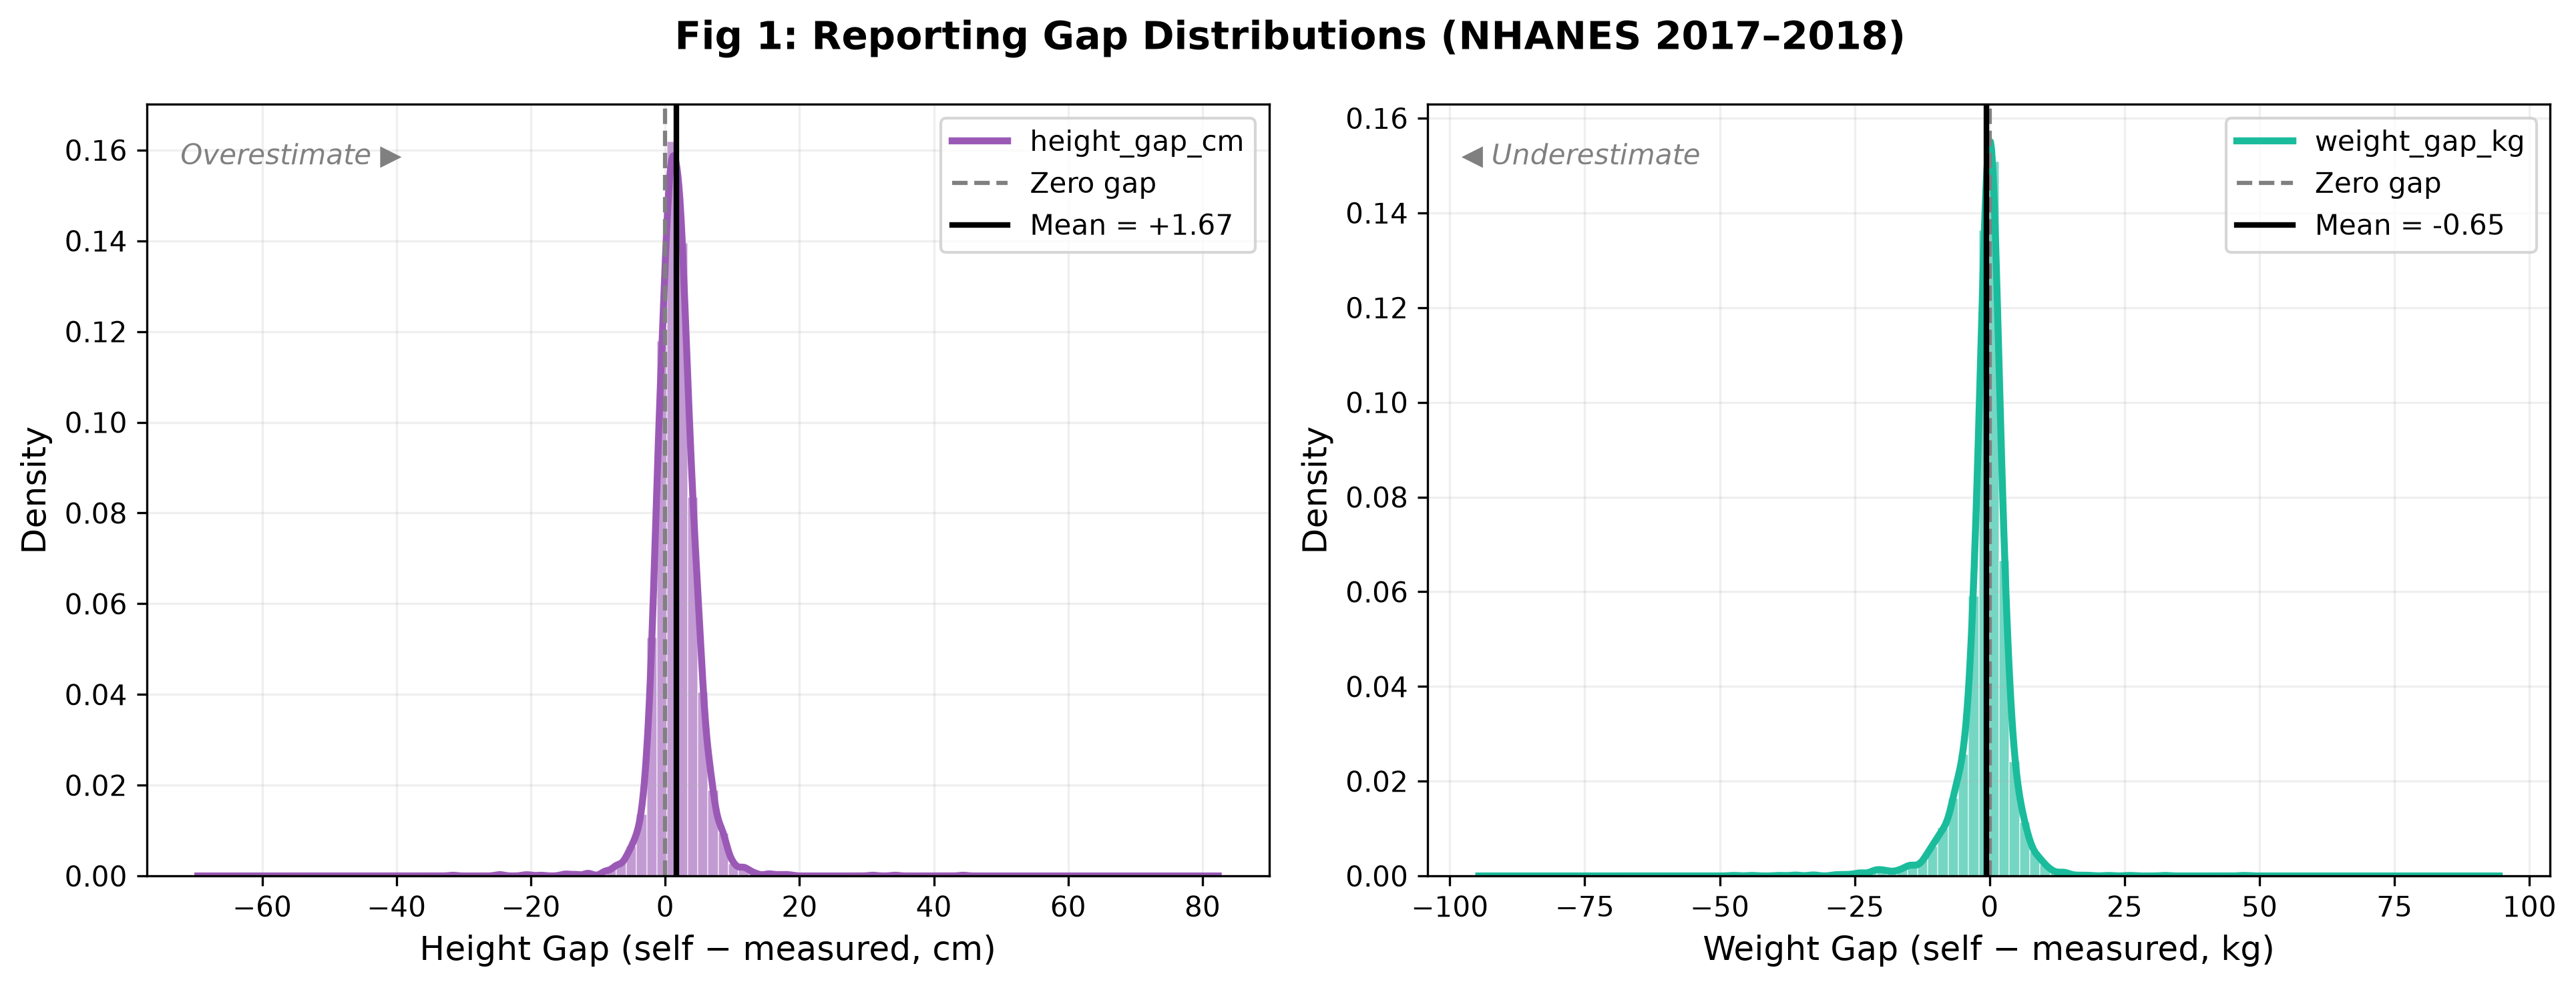
\includegraphics[width=\linewidth]{../results/figures/fig1_reporting_gaps.png}
  \caption{Self-report vs. nurse-measured gap distributions
           (NHANES 2017--2018). Dashed vertical lines indicate
           means; shaded regions mark the 95th-percentile lie budget.}
  \label{fig:gaps}
\end{figure}

\subsection{Main Result: Explanation Equivalence}

Table~\ref{tab:main_results} and Figure~\ref{fig:main_result} show
$N^*$ across all eight configurations.

\begin{table}[t]
  \centering
  \caption{Explanation equivalence $N^*$ across all configurations.
           Values in brackets are 95\% bootstrap CIs.}
  \label{tab:main_results}
  % FILL: paste from results/tables/table4_main_results.csv after Stage 7
  \begin{table}[htbp]
  \centering
  \caption{Main Results: Explanation Equivalence N* Across All 8 Configurations}
  \label{tab:main_results}
  \small
  \begin{tabular}{lrrrrrrrrrr}
    \hline
    Config & Input & Model & Expl. & N patients & Mean N* & 95% CI & Median N* & Std & % Useless & % Worth 10+ \\
    \hline
    reported_rf_shap & Reported & RF & SHAP & 884 & 12.43 & [10.54, 14.53] & 0.0 & 30.21 & 63.8% & 17.2% \\
    reported_rf_lime & Reported & RF & LIME & 884 & 9.41 & [7.66, 11.27] & 0.0 & 26.57 & 67.9% & 12.6% \\
    reported_lr_shap & Reported & LR & SHAP & 884 & 22.77 & [20.36, 25.28] & 0.0 & 38.59 & 59.0% & 32.5% \\
    reported_lr_lime & Reported & LR & LIME & 884 & 22.71 & [20.28, 25.26] & 0.0 & 38.15 & 55.1% & 33.4% \\
    measured_rf_shap & Measured & RF & SHAP & 884 & 10.27 & [8.42, 12.15] & 0.0 & 27.94 & 69.2% & 13.5% \\
    measured_rf_lime & Measured & RF & LIME & 884 & 9.01 & [7.32, 10.77] & 0.0 & 26.49 & 69.8% & 11.8% \\
    measured_lr_shap & Measured & LR & SHAP & 884 & 23.05 & [20.58, 25.61] & 0.0 & 38.78 & 57.1% & 33.3% \\
    measured_lr_lime & Measured & LR & LIME & 884 & 21.27 & [18.99, 23.71] & 0.0 & 37.43 & 56.7% & 30.9% \\
    \hline
  \end{tabular}
\end{table}
\end{table}

\begin{figure}[t]
  \centering
  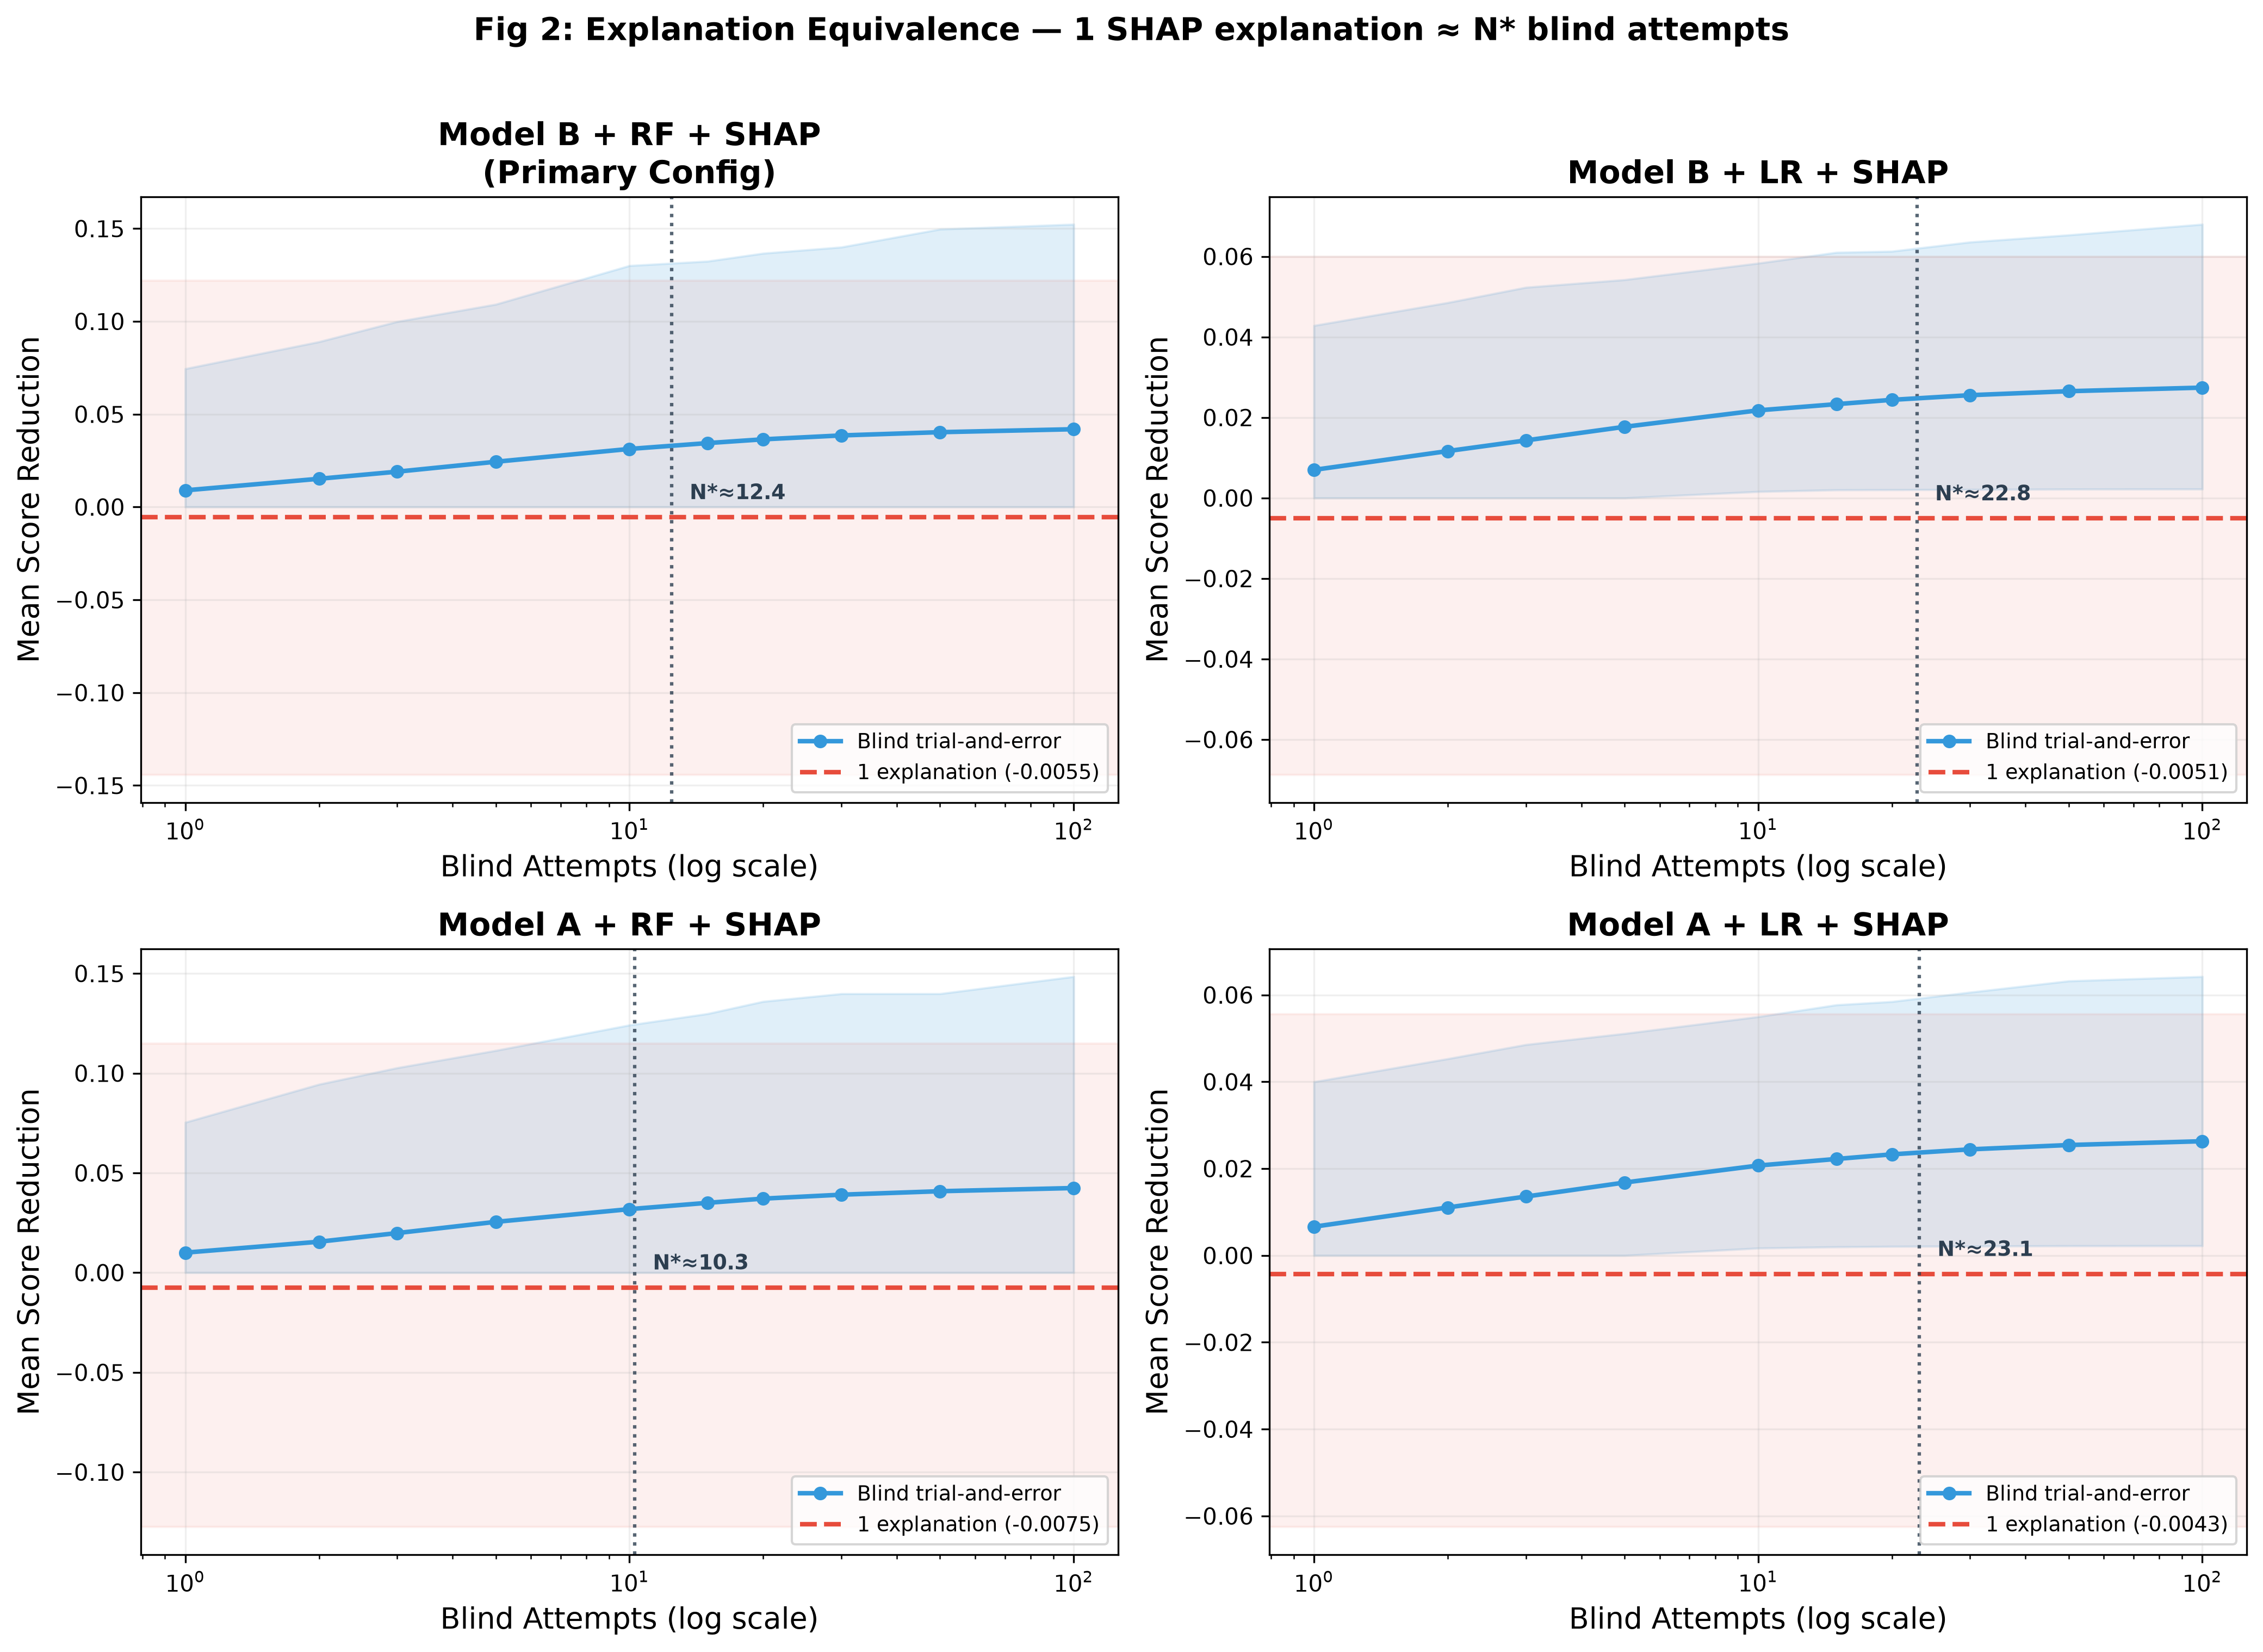
\includegraphics[width=\linewidth]{../results/figures/fig2_main_result.png}
  \caption{Equivalence curves: mean blind score reduction (blue, with
           95\% band) vs.\ explanation reduction (red dashed).
           The crossing point marks $N^*$.}
  \label{fig:main_result}
\end{figure}

\subsection{Per-Patient Distribution}

Figure~\ref{fig:hist} shows the distribution of per-patient $N^*$.
For [X]\% of patients, the explanation provides no benefit over a
single blind query ($N^* \leq 1$).  For [Y]\% of patients, the
explanation is worth more than 10 blind attempts ($N^* \geq 10$).

\begin{figure}[t]
  \centering
  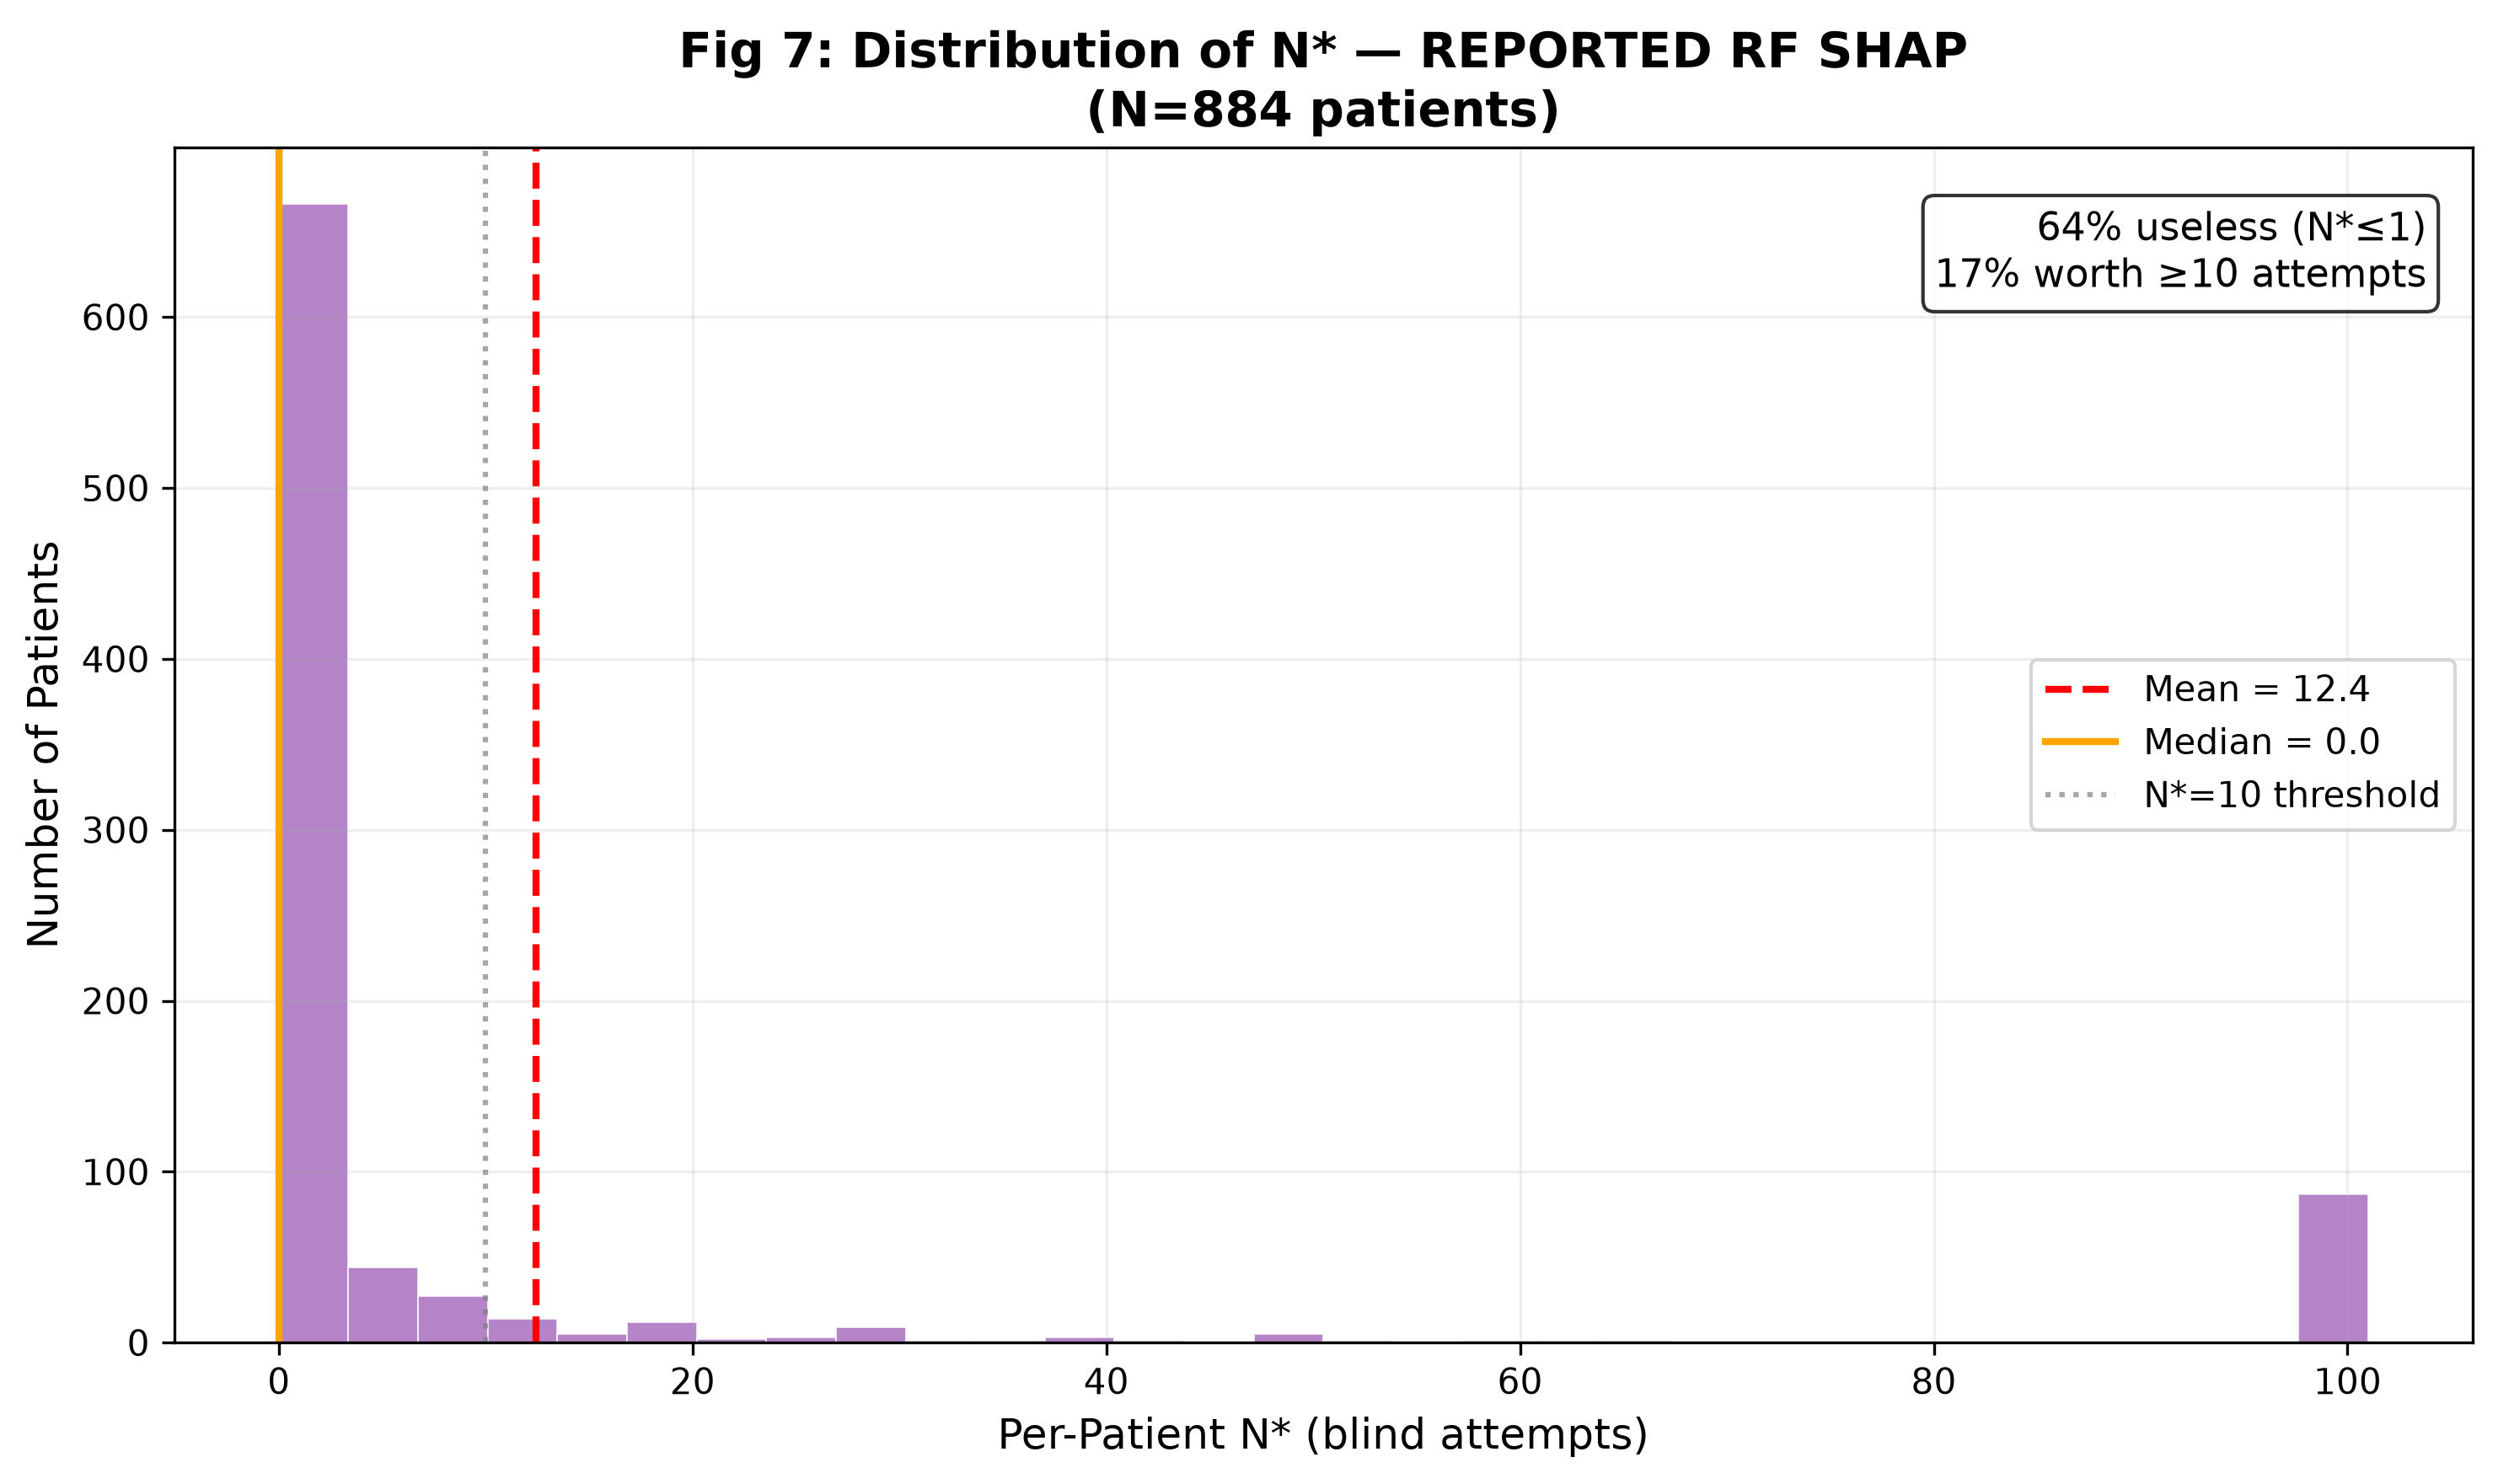
\includegraphics[width=\linewidth]{../results/figures/fig7_nstar_histogram.png}
  \caption{Distribution of per-patient equivalence $N^*$
           (reported RF + SHAP; $N=[X]$ patients).}
  \label{fig:hist}
\end{figure}

\subsection{Model A vs.\ Model B}

Figure~\ref{fig:modelab} compares $N^*$ for models trained on
nurse-measured (Model A) vs.\ self-reported (Model B) inputs.  [FILL
interpretation after results].

\subsection{SHAP vs.\ LIME Agreement}

Figure~\ref{fig:scatter} shows $N^*_{\text{SHAP}}$ vs.\
$N^*_{\text{LIME}}$ for each configuration.
[FILL: close to diagonal = methods agree].

\subsection{Statistical Tests}

Table~\ref{tab:stats} reports Wilcoxon $p$-values and Cohen's $d$
for the comparison explanation vs.\ blind at $N=10$ across all
configurations.  [FILL: $p < 0.05$ / not significant?].

% ============================================================
\section{Discussion}
% ============================================================

% --- TODO (Akshat Kumar, Week 4) ---------------------------
% 1 page. Sub-sections:
%   6.1 Main takeaway: what N* means for policy
%   6.2 If N* < 5: "restricting explanations is not the solution"
%   6.3 If N* 5-20: "moderate risk, consider design countermeasures"
%   6.4 If N* > 20: "explanations are powerful; anonymise or restrict"
%   6.5 Limitations
%   6.6 Recommendations for practitioners

\subsection{Policy Implications}

Based on our pre-registered interpretation guide:
\begin{itemize}
  \item \textbf{If $N^* < 5$}: Withholding explanations is not a
        meaningful safeguard.  A patient who is motivated to game the
        model can do so almost as effectively through blind
        trial-and-error.  The benefit of transparency outweighs the
        gaming risk.
  \item \textbf{If $5 \leq N^* \leq 20$}: Explanations provide a
        moderate gaming advantage.  Design-level countermeasures---such
        as rate-limiting queries or adding perturbation noise---are
        worth considering.
  \item \textbf{If $N^* > 20$}: Explanations are powerful attack
        vectors.  Restricting or anonymising explanations may be
        warranted; input verification (e.g., nurse measurement) is the
        more robust safeguard.
\end{itemize}

Our result of $N^* \approx [FILL]$ falls in the [FILL] category,
suggesting [FILL interpretation].

\subsection{Limitations}

\begin{itemize}
  \item \textbf{Single domain.} Our study is limited to diabetes risk
        from anthropometric self-report. Results may differ for other
        clinical domains or feature types.
  \item \textbf{Single-feature attack.} We model an adversary who
        changes one feature optimally (explanation-guided) or randomly
        (blind). Multi-feature attacks could be more powerful.
  \item \textbf{Static model.} We assume the model does not adapt to
        gaming attempts. Adversarially robust training is a complementary
        defence.
  \item \textbf{Lie budget from observational data.} The 95th-percentile
        gap captures what people \emph{actually} misreport, not the
        maximum they \emph{could} misreport.
\end{itemize}

\subsection{Recommendations for Practitioners}

\begin{enumerate}
  \item Prefer \textbf{verified inputs} (nurse measurement) over
        self-report for high-stakes predictions.
  \item If explanations must be shown, \textbf{rate-limit queries}
        to raise the cost of blind trial-and-error.
  \item Audit models for gaming vulnerability before deployment using
        the $N^*$ framework introduced here.
  \item Pre-register your evaluation plan to build trust in empirical
        findings.
\end{enumerate}

% ============================================================
\section{Conclusion}
% ============================================================

% --- TODO (Akash Singh, Week 4) ---------------------------
% 0.5 page: summarise, state N*, restate policy conclusion, future work

We introduced the \emph{explanation equivalence} metric $N^*$ and
applied it to a diabetes risk model using real NHANES survey data.
Our pre-registered experiment on held-out 2017--2018 data shows that
one SHAP explanation is equivalent to approximately $N^*$ [FILL] blind
attempts (95\% CI: $L$--$H$).  This quantifies, for the first time in
a realistic clinical setting, the gaming advantage conferred by an XAI
explanation.

Our result suggests that [small/moderate/large]: [FILL conclusion].
The most effective safeguard against gaming clinical AI systems is
verifying self-reported inputs rather than withholding explanations.

\paragraph{Future Work.}
Extensions include multi-feature adversarial attacks, adaptive model
defences, other clinical domains, and evaluation of counterfactual
explanation methods.

% ============================================================
% REFERENCES
% ============================================================

\bibliographystyle{ACM-Reference-Format}
\bibliography{references}

\end{document}
